\documentclass{article}
\usepackage[english]{babel}
\usepackage{amsmath, amssymb, graphicx}
\DeclareMathOperator*{\argmax}{argmax}
\graphicspath{{./images/}}


\title{CPS841 Reinforcement Learning - Assignment 1}
\author{Nariman Saftarli - nsaftarli@ryerson.ca}

\begin{document}
\maketitle
\newpage

Question 1.  Both the UCB algorithm as well as the $\epsilon$-greedy algorithm were implemented, the latter as a baseline. Running each algorithm for $100,000$ rounds, the following observations were made:
	\begin{enumerate}
	\item For both the UCB algorithm as well as the $\epsilon$-greedy algorithm, the real probability distribution and estimated probability distribution were plotted. The results were as expected. As the focus is to select the option with the highest chance of receiving a reward, the estimated probability distribution does not generally accurately represent the true probability distribution for any more than 1 of 10 values where 10 represents the number of actions that can be taken in the 10-armed bandit problem. This is because there's no motivation other than maximizing the reward signal over time, which makes low-valued actions irrelevant over time, and predicting their actual probabilities is unnecessary; all that's necessary is to confirm that they are not optimal. Figure 1 illustrates this. There are two things important to note here. The first is that the estimated probability is acceptably accurate for a \textit{single} value in the distribution (\textit{i.e.} the peak of the estimated probability distribution is reasonably close to the actual value at that index in the true probability distribution). The second is that the $\epsilon$-greedy method failed at finding the optimal move.
	\begin{figure}[h]
	\centering
	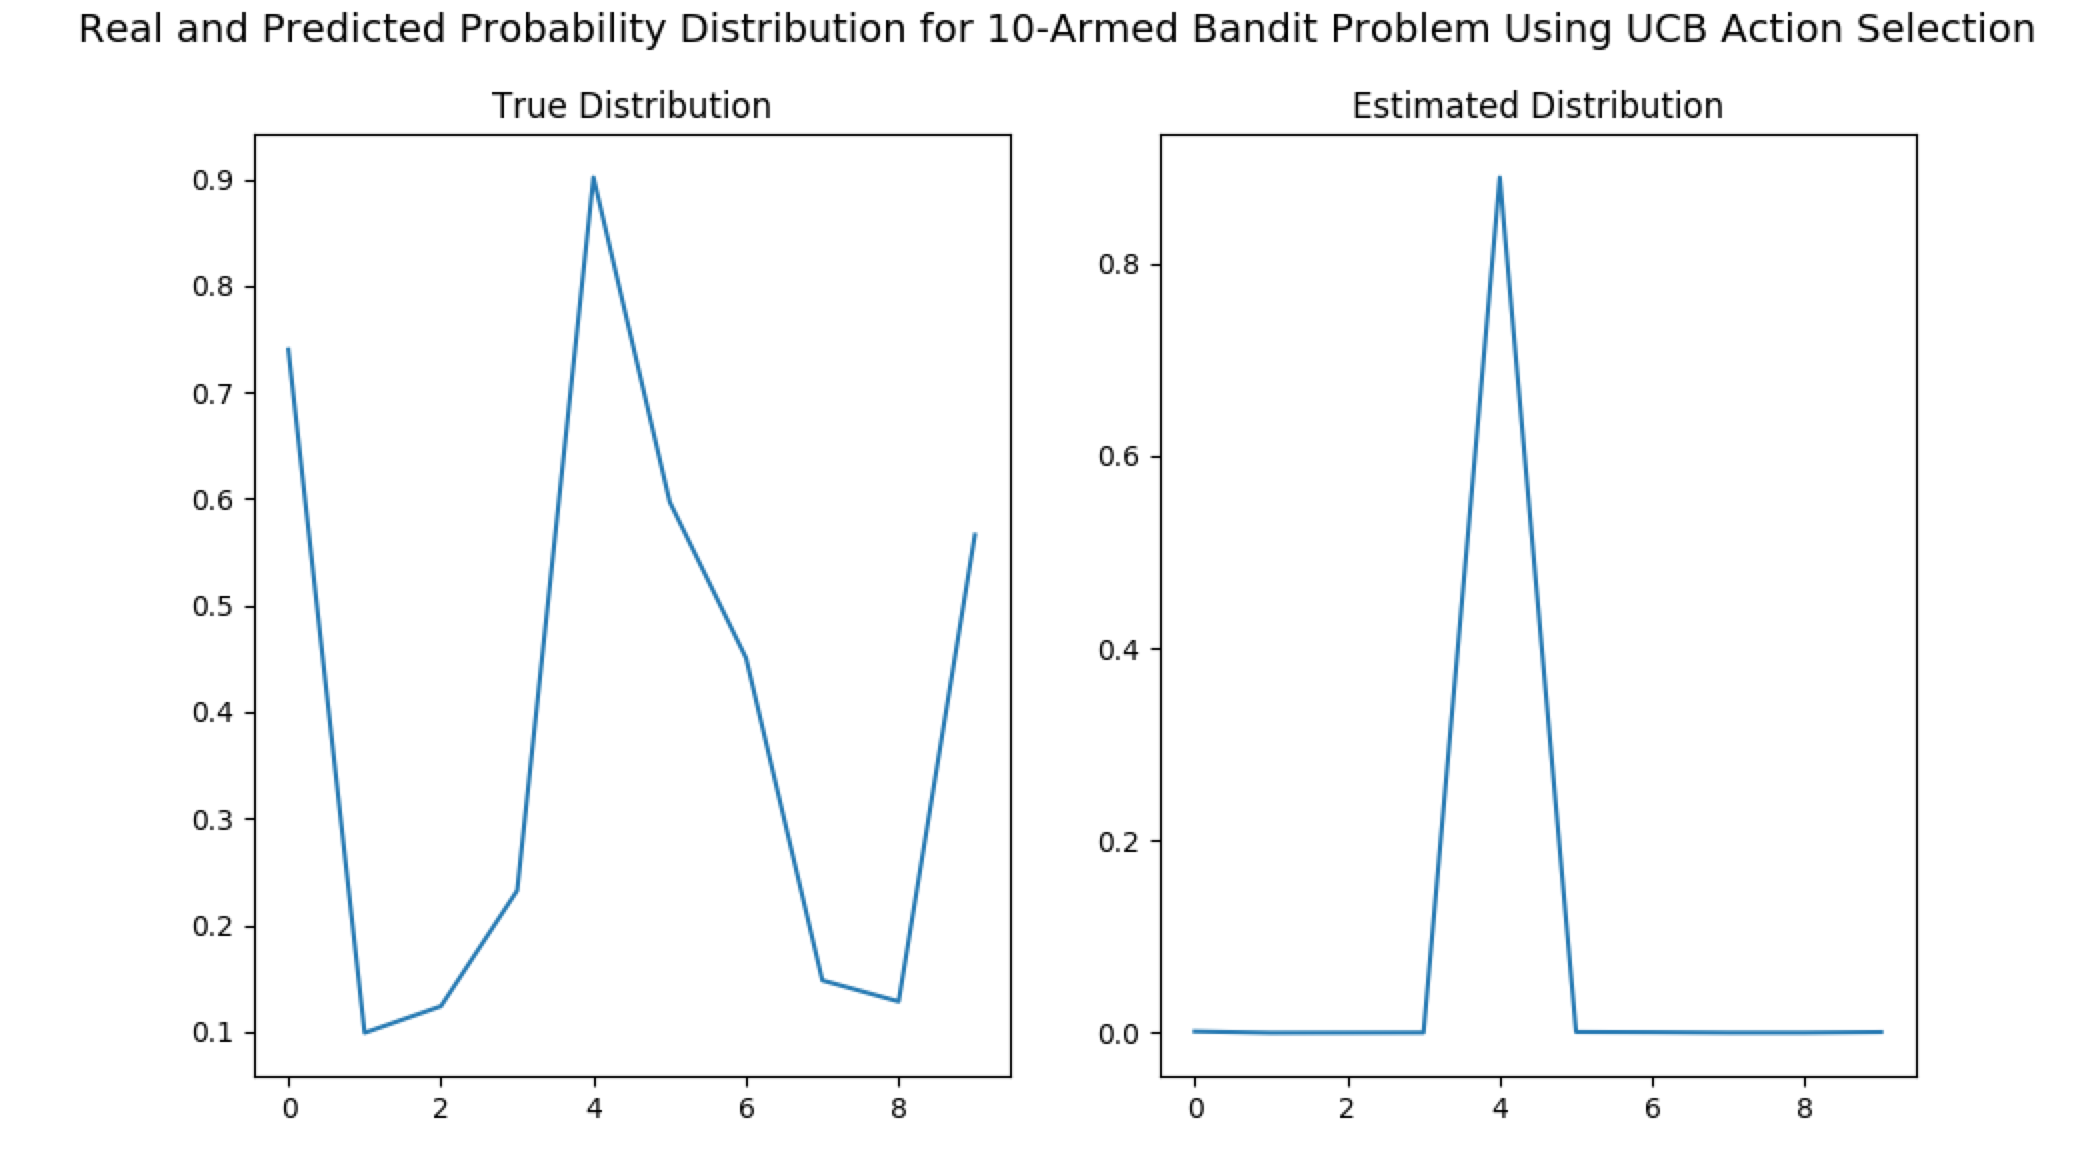
\includegraphics[scale=0.2]{ucb_pred}
	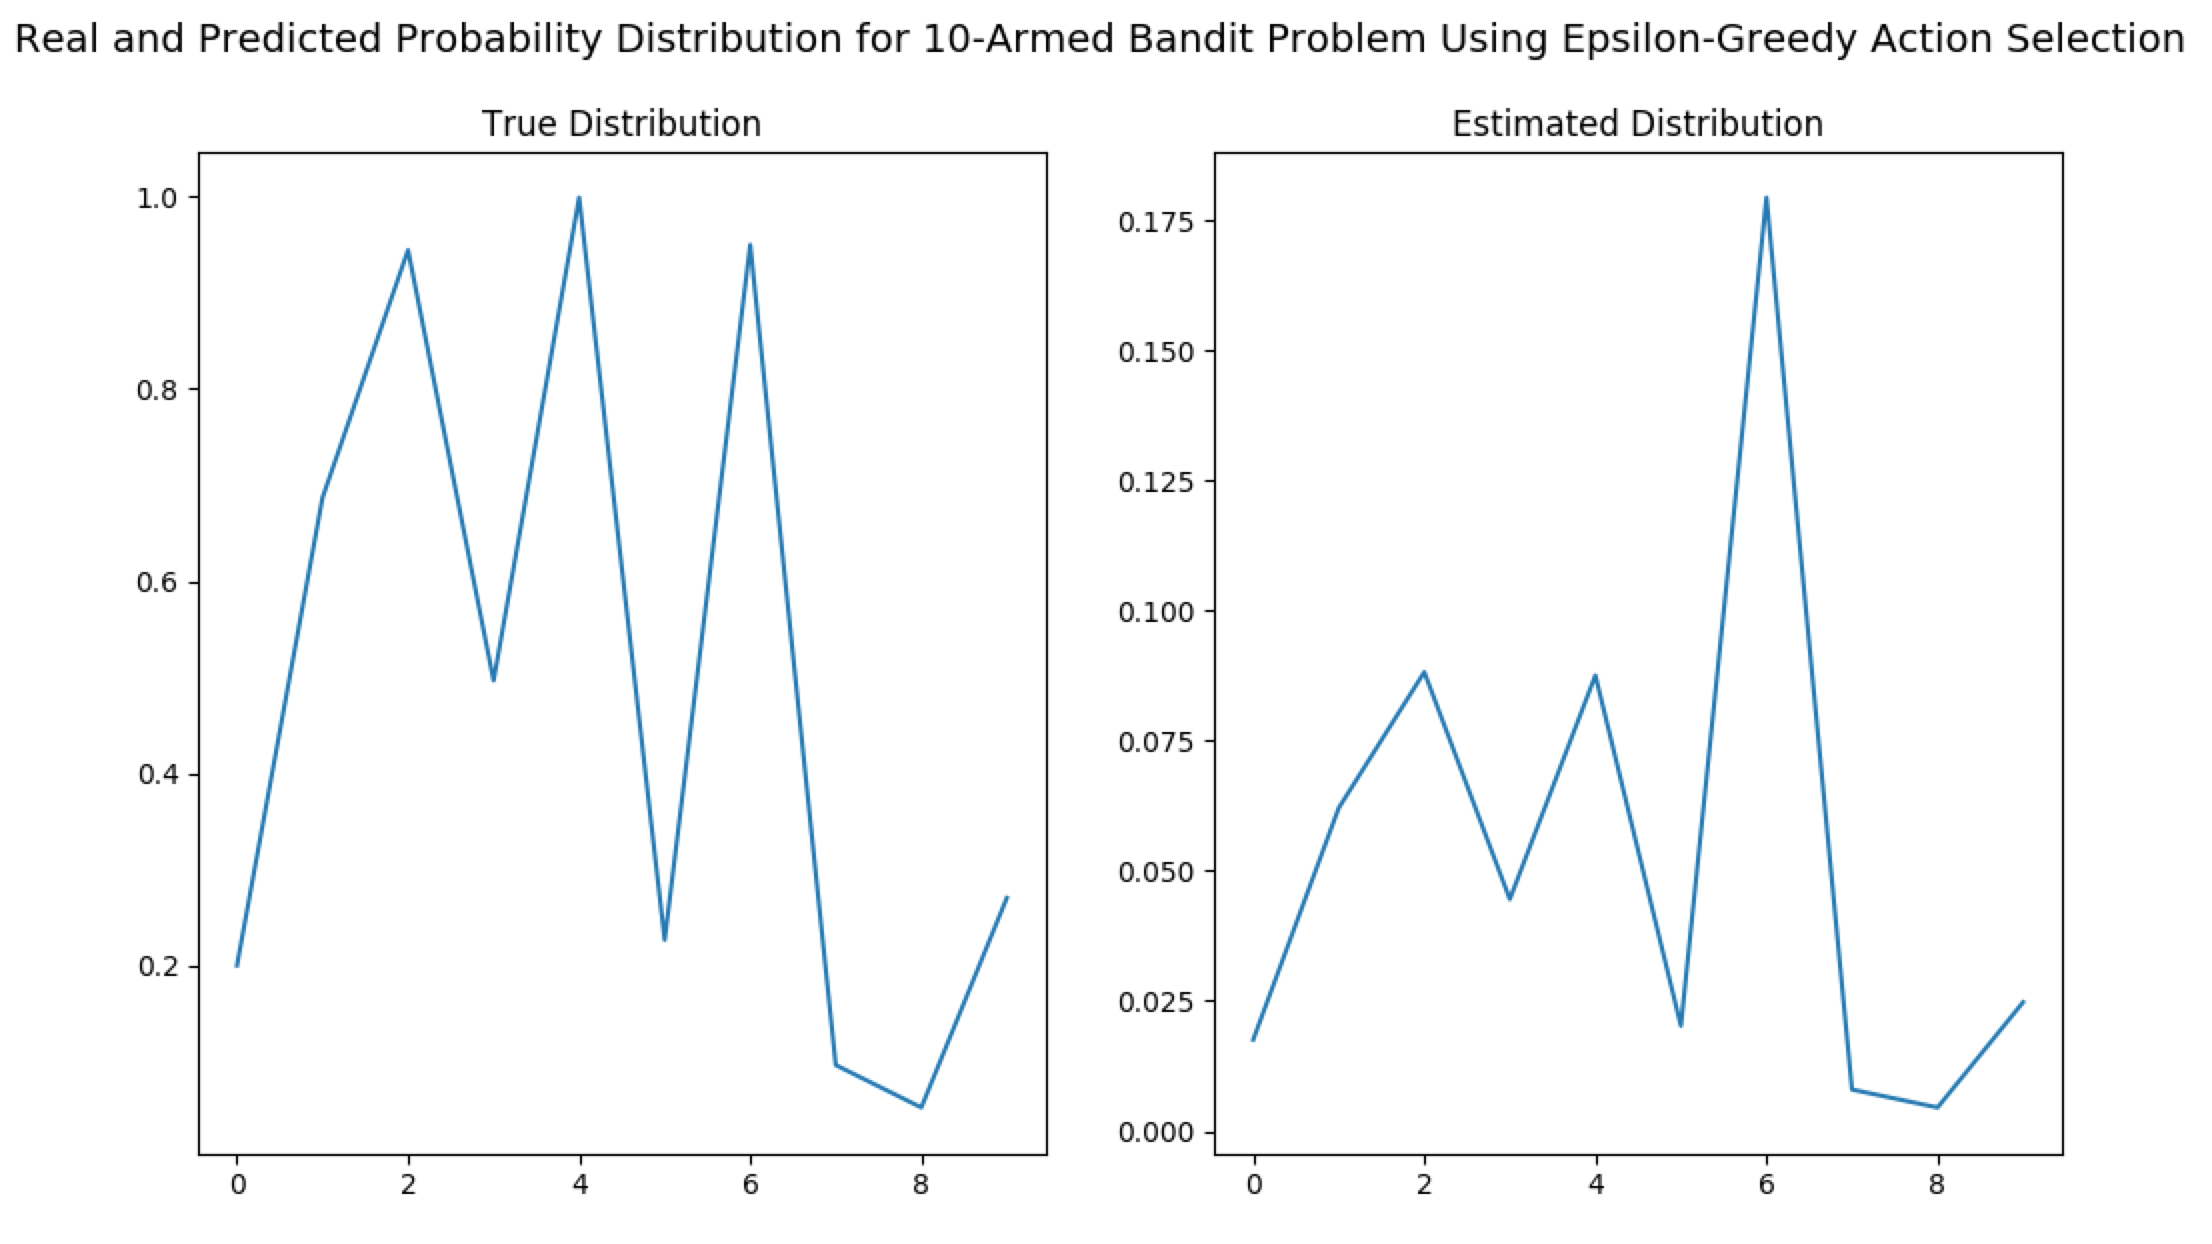
\includegraphics[scale=0.2]{eps_pred}
	\caption{Both the UCB and $\epsilon$-greedy algorithms predict the entire distribution incorrectly, but fairly accurately approximate a single probability.}
	\end{figure}
	\item The UCB algorithm converged on the optimal action much more reliably in the 10-armed bandit problem than did the $\epsilon$-greedy algorithm. This also makes sense since the $\epsilon$-greedy algorithm fails to have some measure of uncertainty. That is, if $\epsilon=0.9$, and some action produces a positive reward, the $\epsilon$-greedy algorithm is much more likely to choose that value and get stuck at a local optimum, because there's nothing to specify its uncertainty about the potential of other values to yield a high reward. This is shown in figure 2, as the algorithm starts off making the optimal action $10\%$ of the time (as expected), but which quickly drops down to $1\%$ as the non-optimal action is chosen more often. The UCB algorithm however increases the rate at which it makes the optimal action. This is because of two major factors. The first is that the UCB algorithm (\textit{i.e.} action selection specified by $A_t = \argmax_x [Q_t(a) + c\sqrt{\frac{lnt}{N_t(a)}}]$ has some notion of uncertainty, while the second makes it such that the degree of uncertainty is decreased over time. 
	\begin{figure}[h]
	\centering
	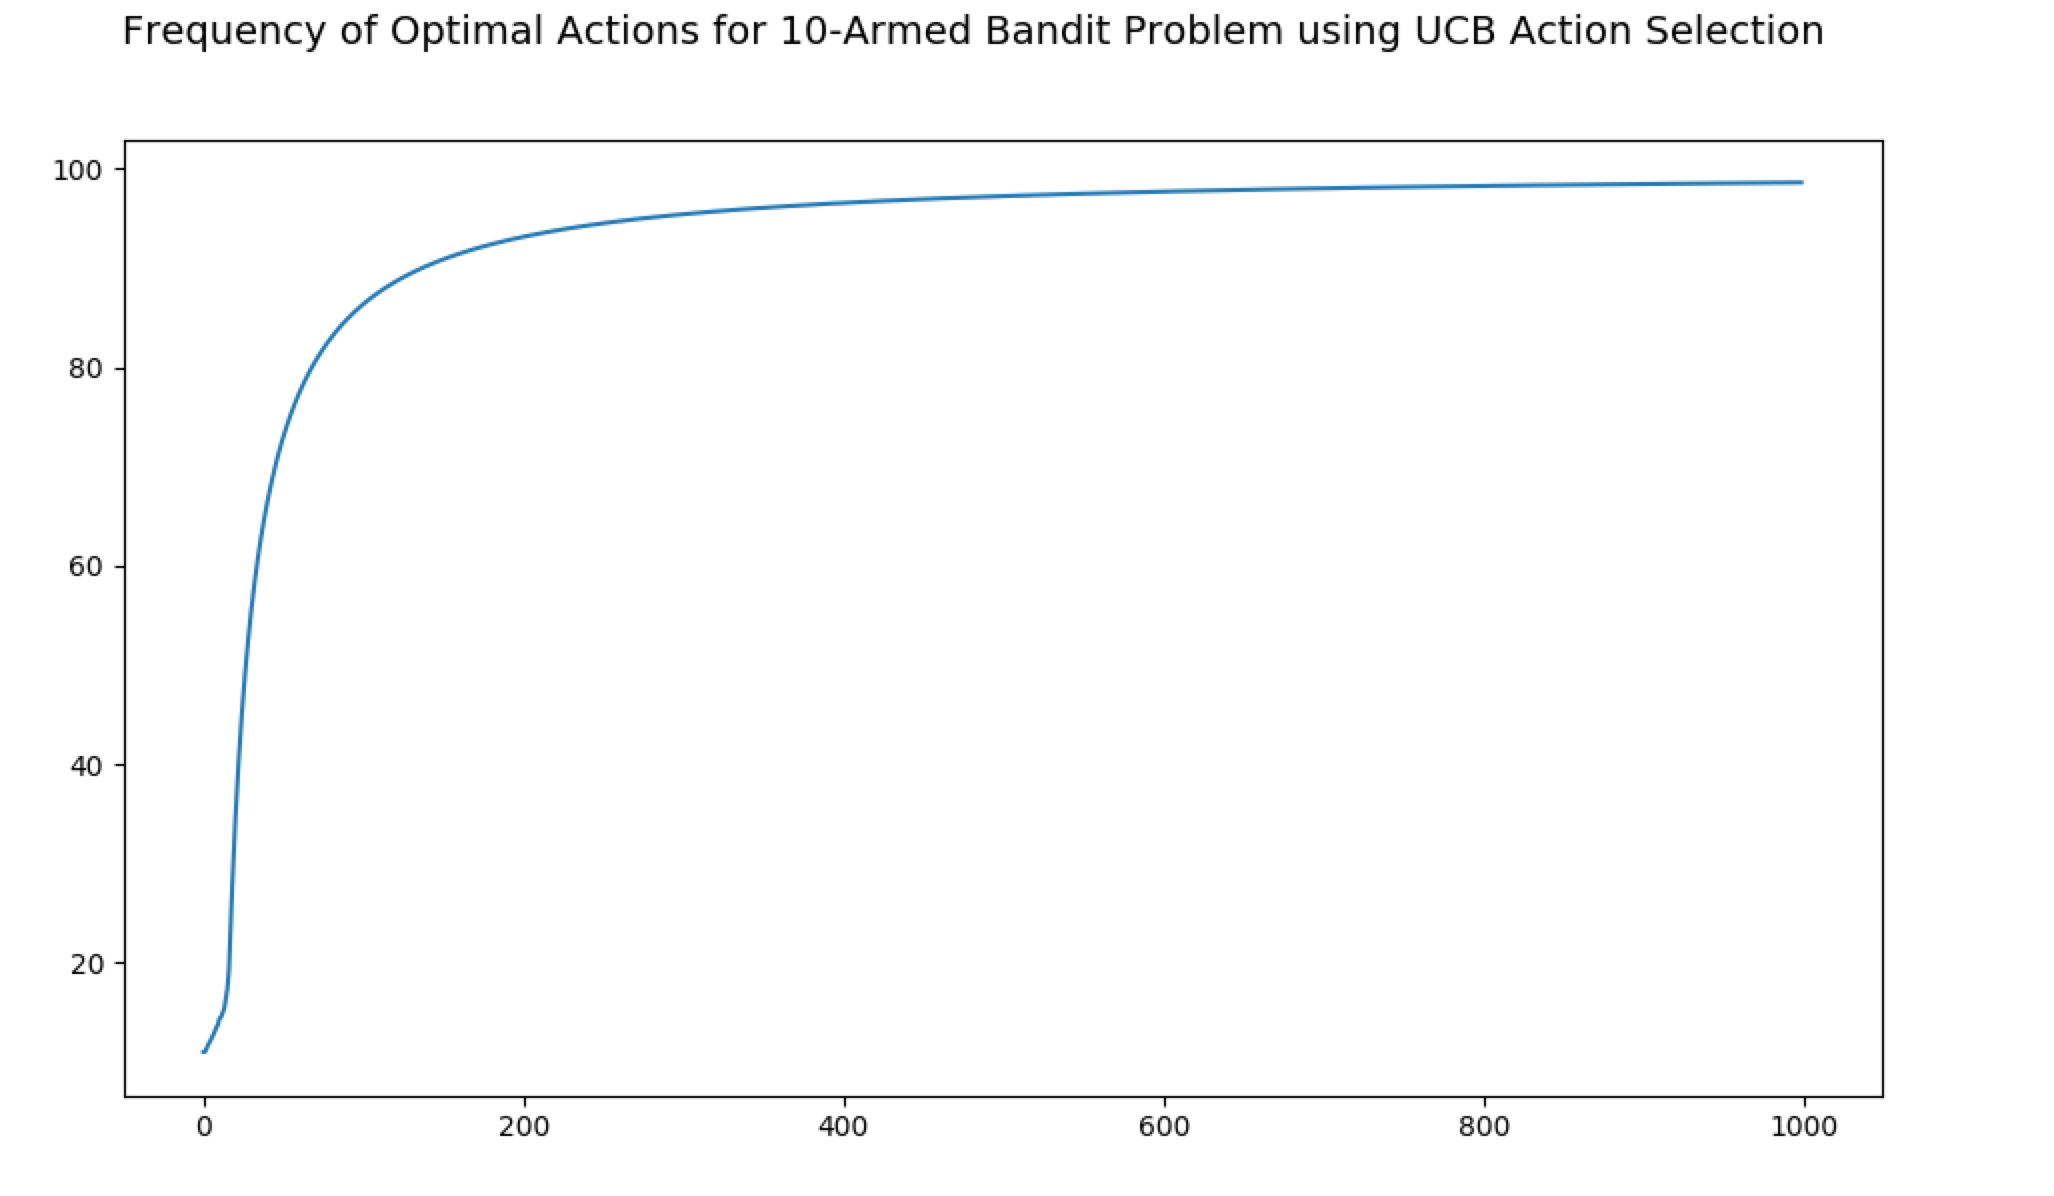
\includegraphics[scale=0.2]{ucb_opt}
	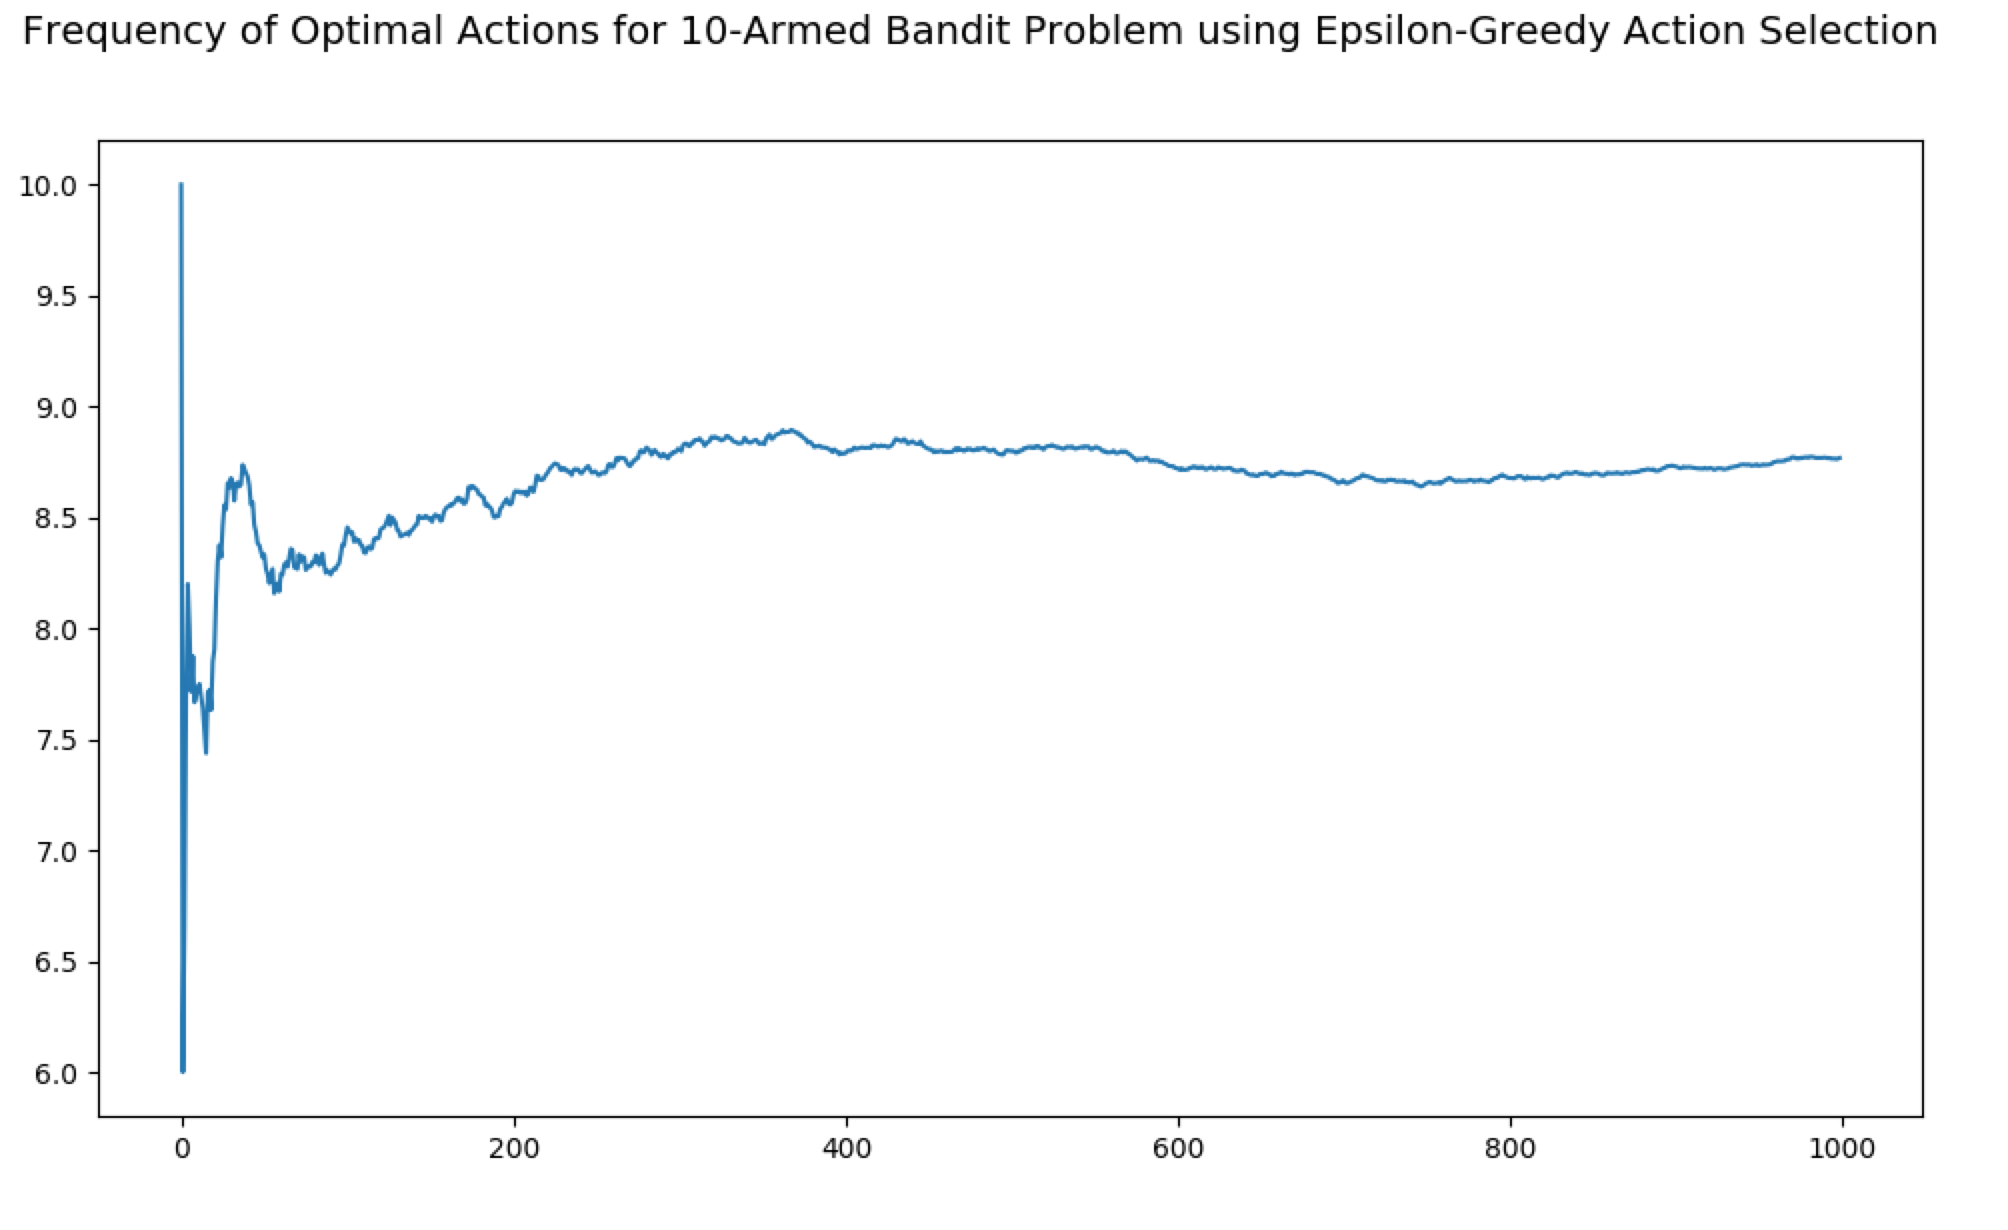
\includegraphics[scale=0.2]{eps_opt}
	\caption{The UCB algorithm quickly converges on making the optimal move, whereas the $\epsilon$-greedy algorithm gets stuck at a local peak.}
	\end{figure}
	\item The UCB algorithm increases average reward over time, getting converging on the highest average reward possible whereas the $\epsilon$-greedy algorithm converges on a lower average reward. This is again due to the fact that the $\epsilon$-greedy algorithm is more likely to pick actions that are local optima. Figure 3 illustrates the convergence of the average reward over time.
	\begin{figure}[h]
	\centering
	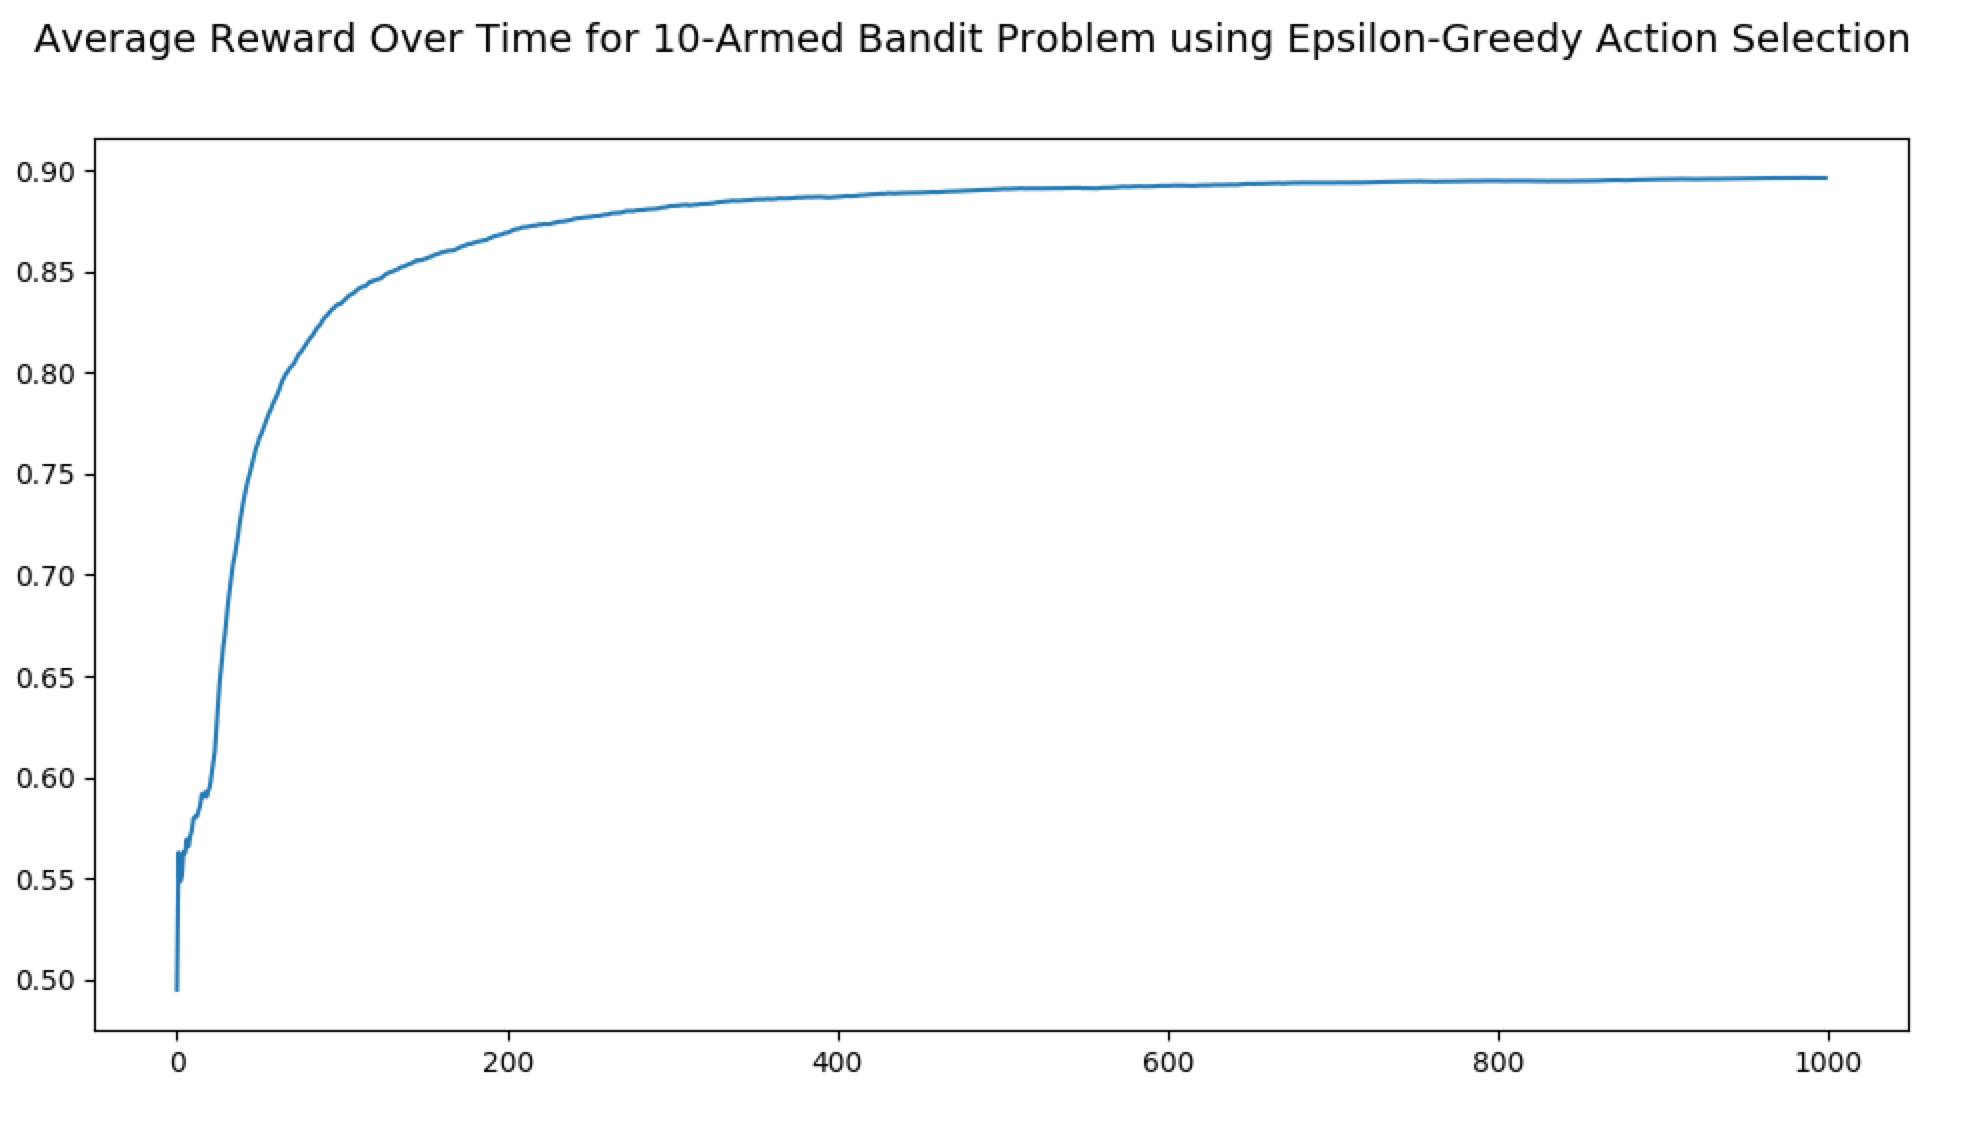
\includegraphics[scale=0.2]{ucb_rew}
	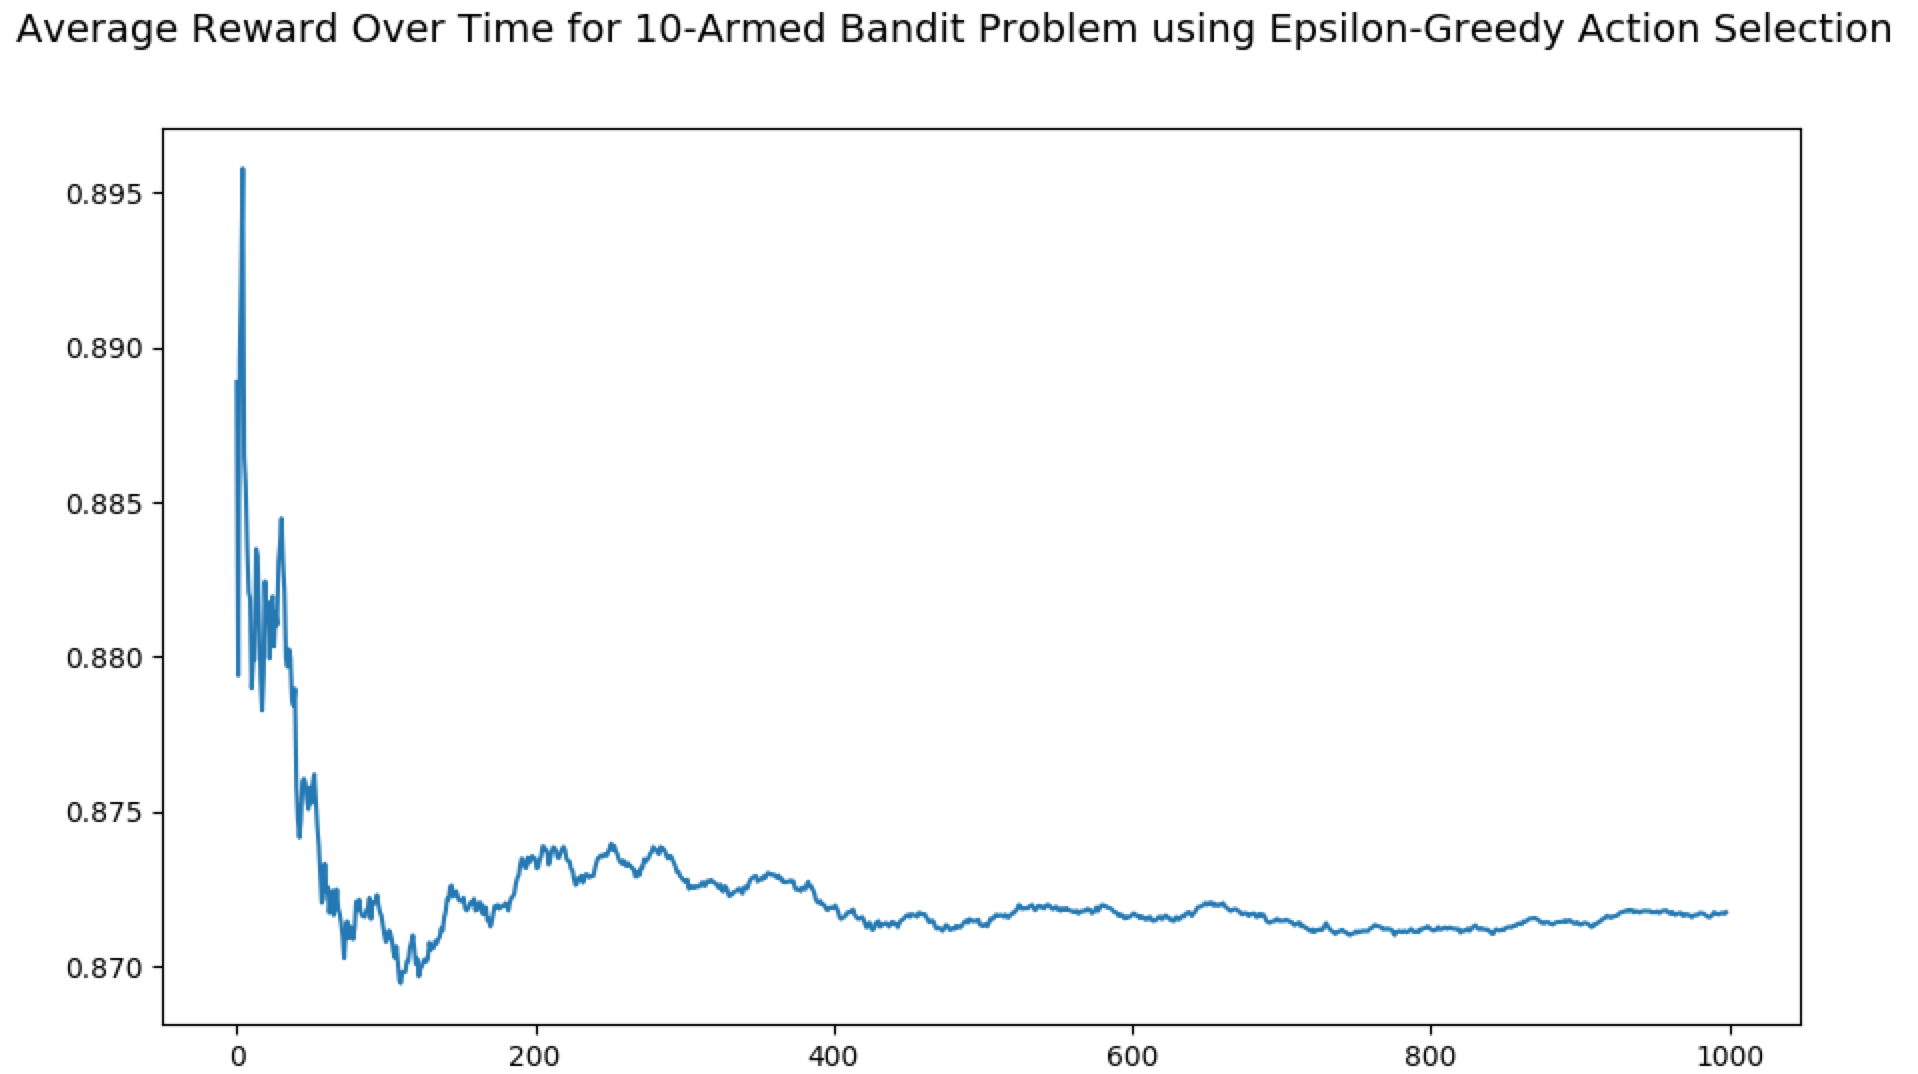
\includegraphics[scale=0.2]{eps_rew}
	\caption{The UCB algorithm converges to a higher average reward than the $\epsilon$-greedy algorithm due to its increased robustness to local optima (making the global action more likely to be chosen over time).}
	\end{figure}
	\end{enumerate}
	
	

	
	
	
Question 2. Both linear and non-linear learning automata were implemented. Running each algorithm for $100,000$ rounds, the following observations were made:
	\begin{enumerate}
	\item The learning rate hyper-parameter (\textit{i.e.} $\alpha$) strongly influenced the convergence and speed of the automata. Specifically, a high learning rate was liable to vary the probabilities heavily, causing the optimal choice percentage to drop and the average reward value to converge to a relatively low value. A low learning rate required more steps to converge but did so more often. A low learning rate also resulted in an action probability distribution that was fairly strongly correlated with the distribution of win probabilities for the $k$-arm bandit, as seen in Figure 4 and 5.
	\begin{figure}[h]
	\centering
	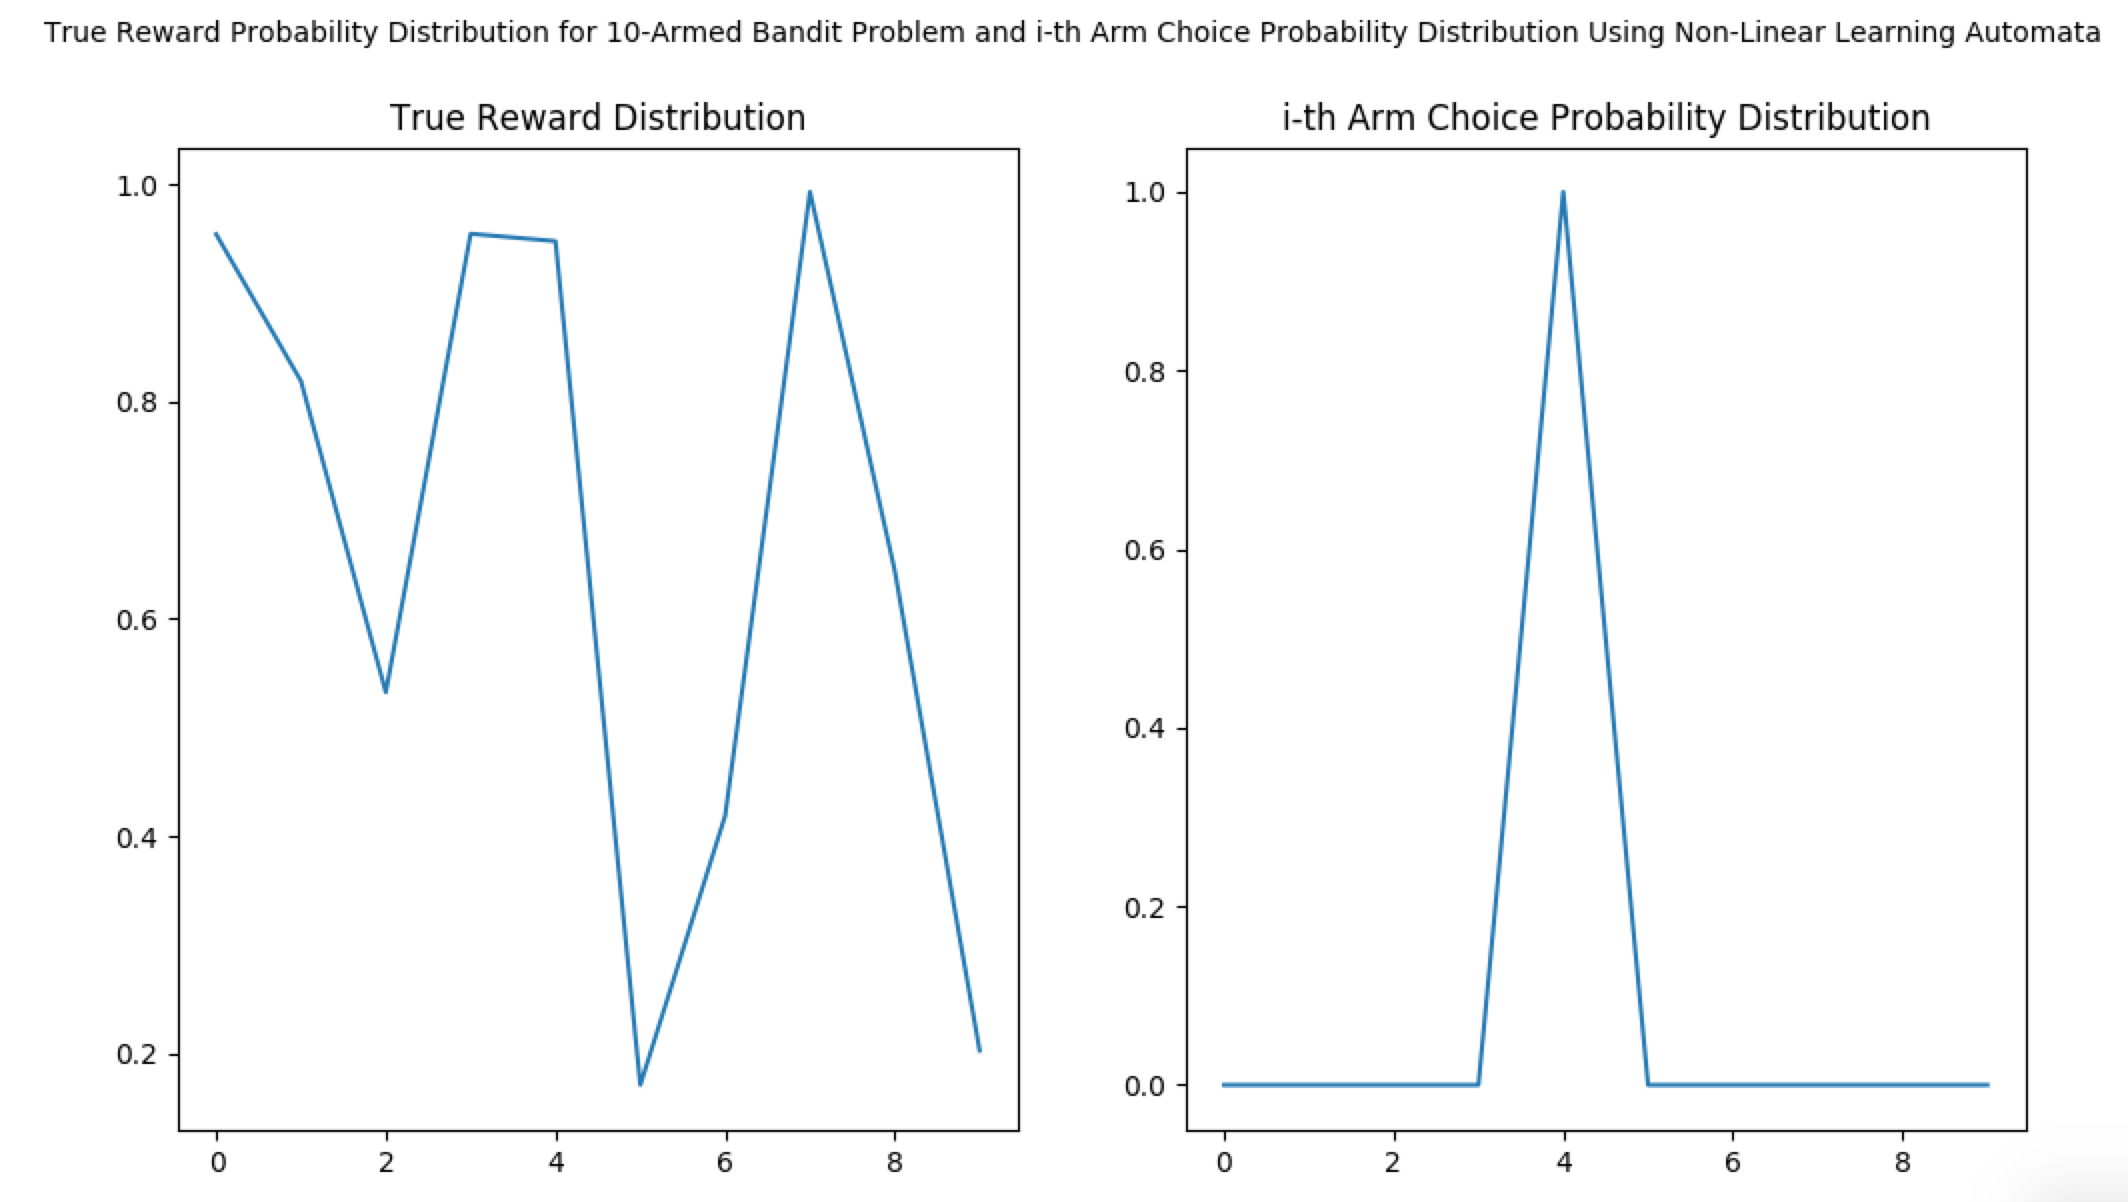
\includegraphics[scale=0.2]{nlla_pred_hlr}
	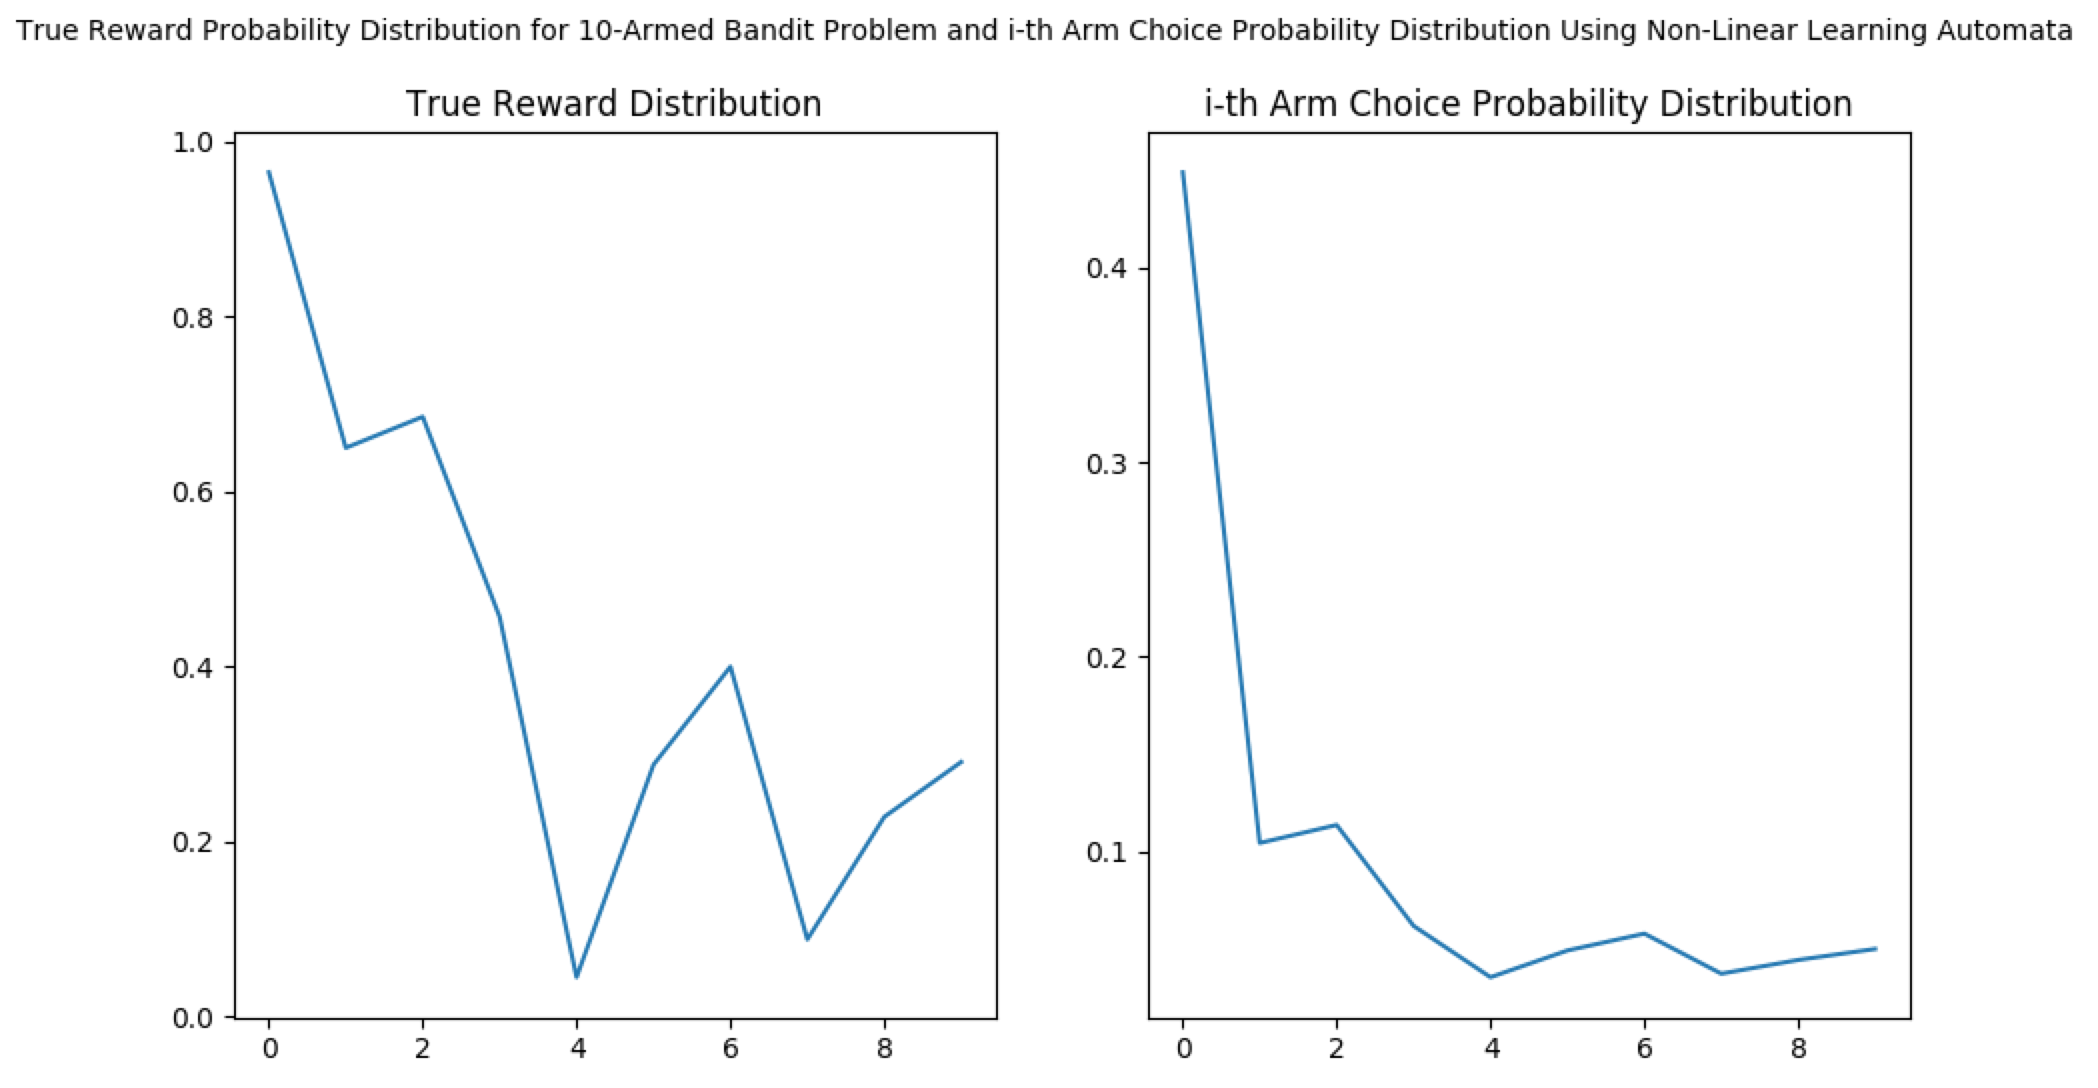
\includegraphics[scale=0.2]{nlla_pred_llr}
	\caption{The probability distribution of actions taken by Non-Linear Learning Automata with a high learning rate ($\alpha=1$, top) and that of actions taken by one with a low learning rate ($\alpha=0.0001$, bottom).}
	\end{figure}
	
	\begin{figure}[h]
	\centering
	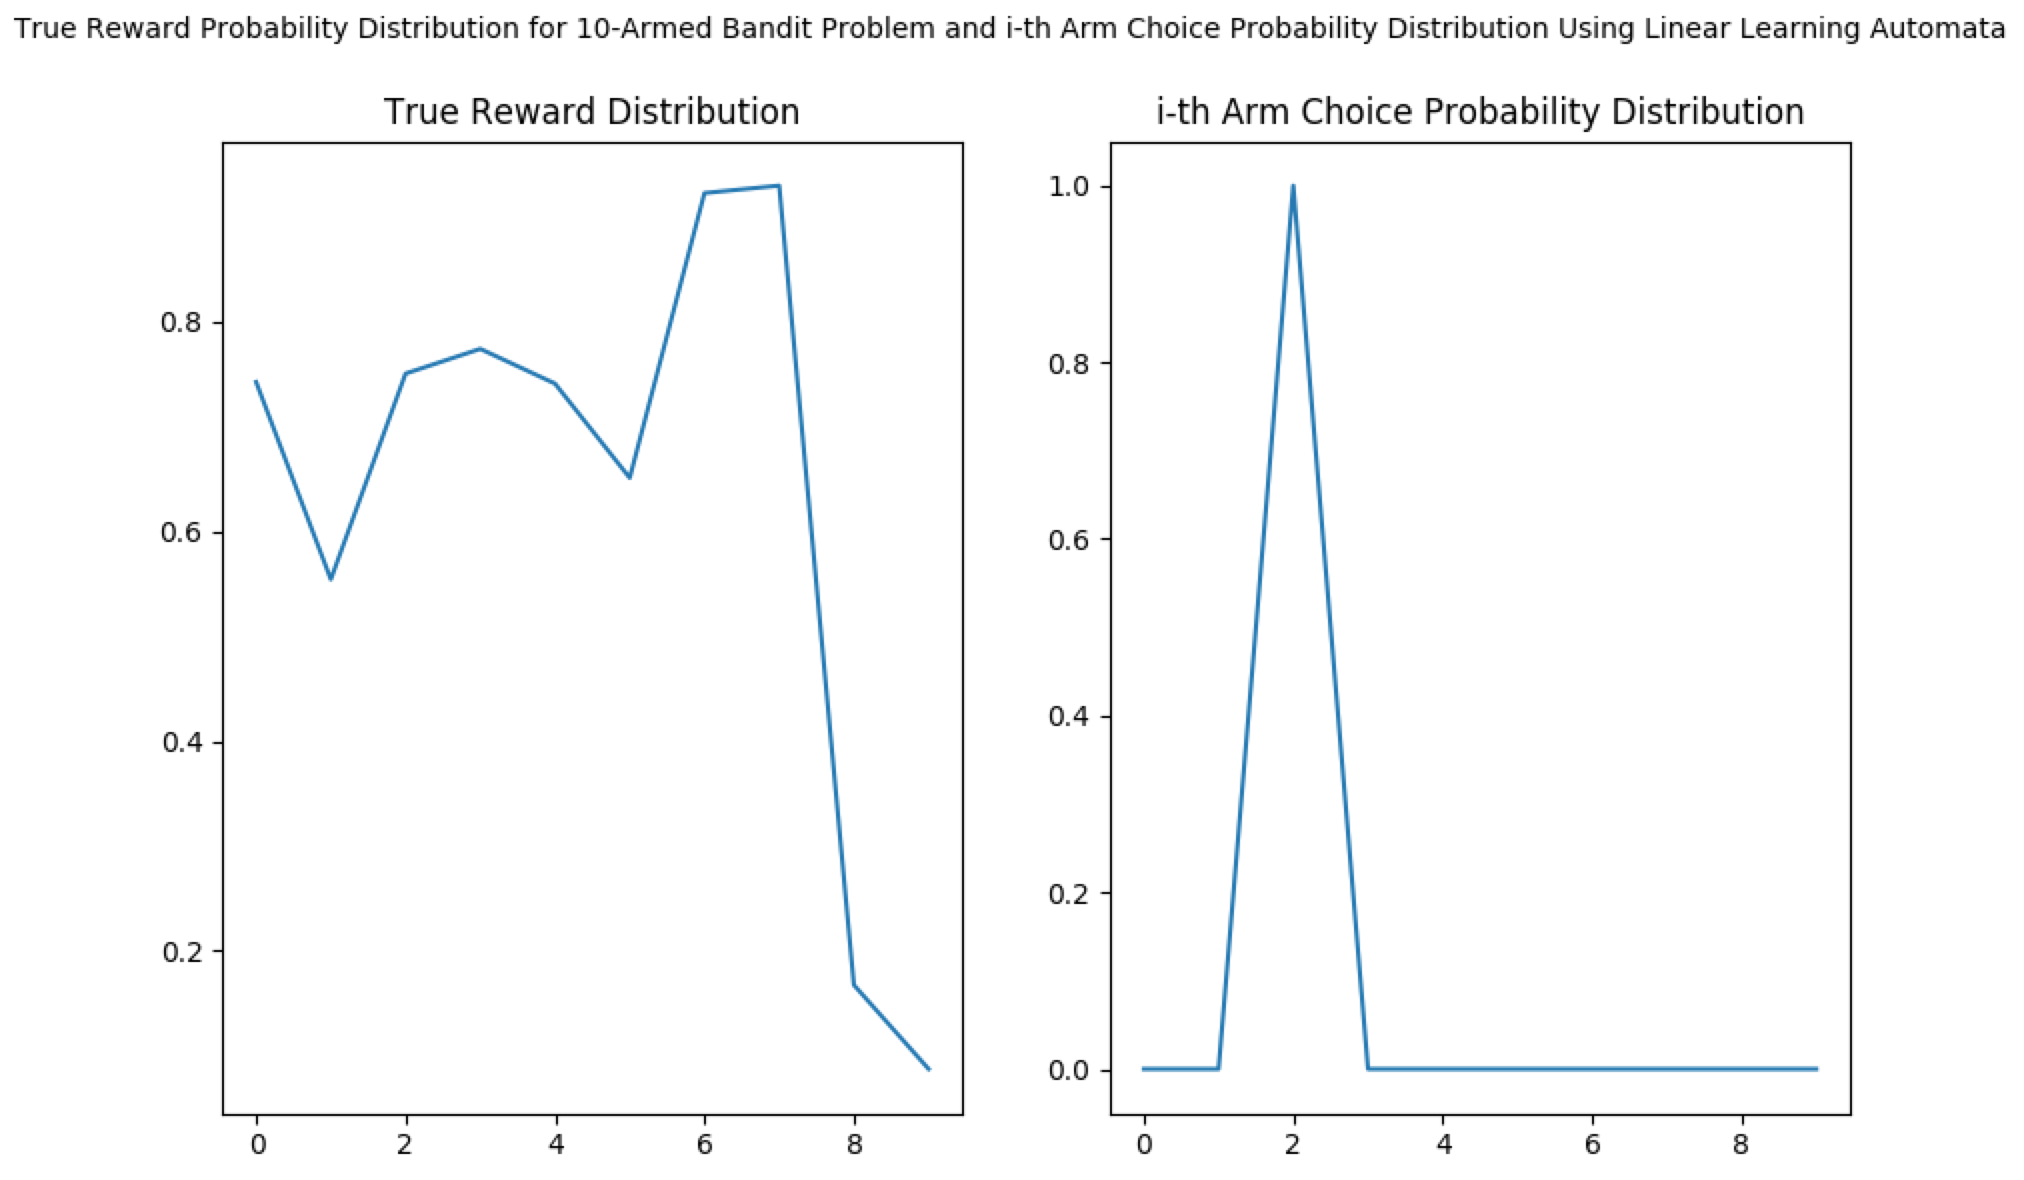
\includegraphics[scale=0.2]{lla_pred_hlr}
	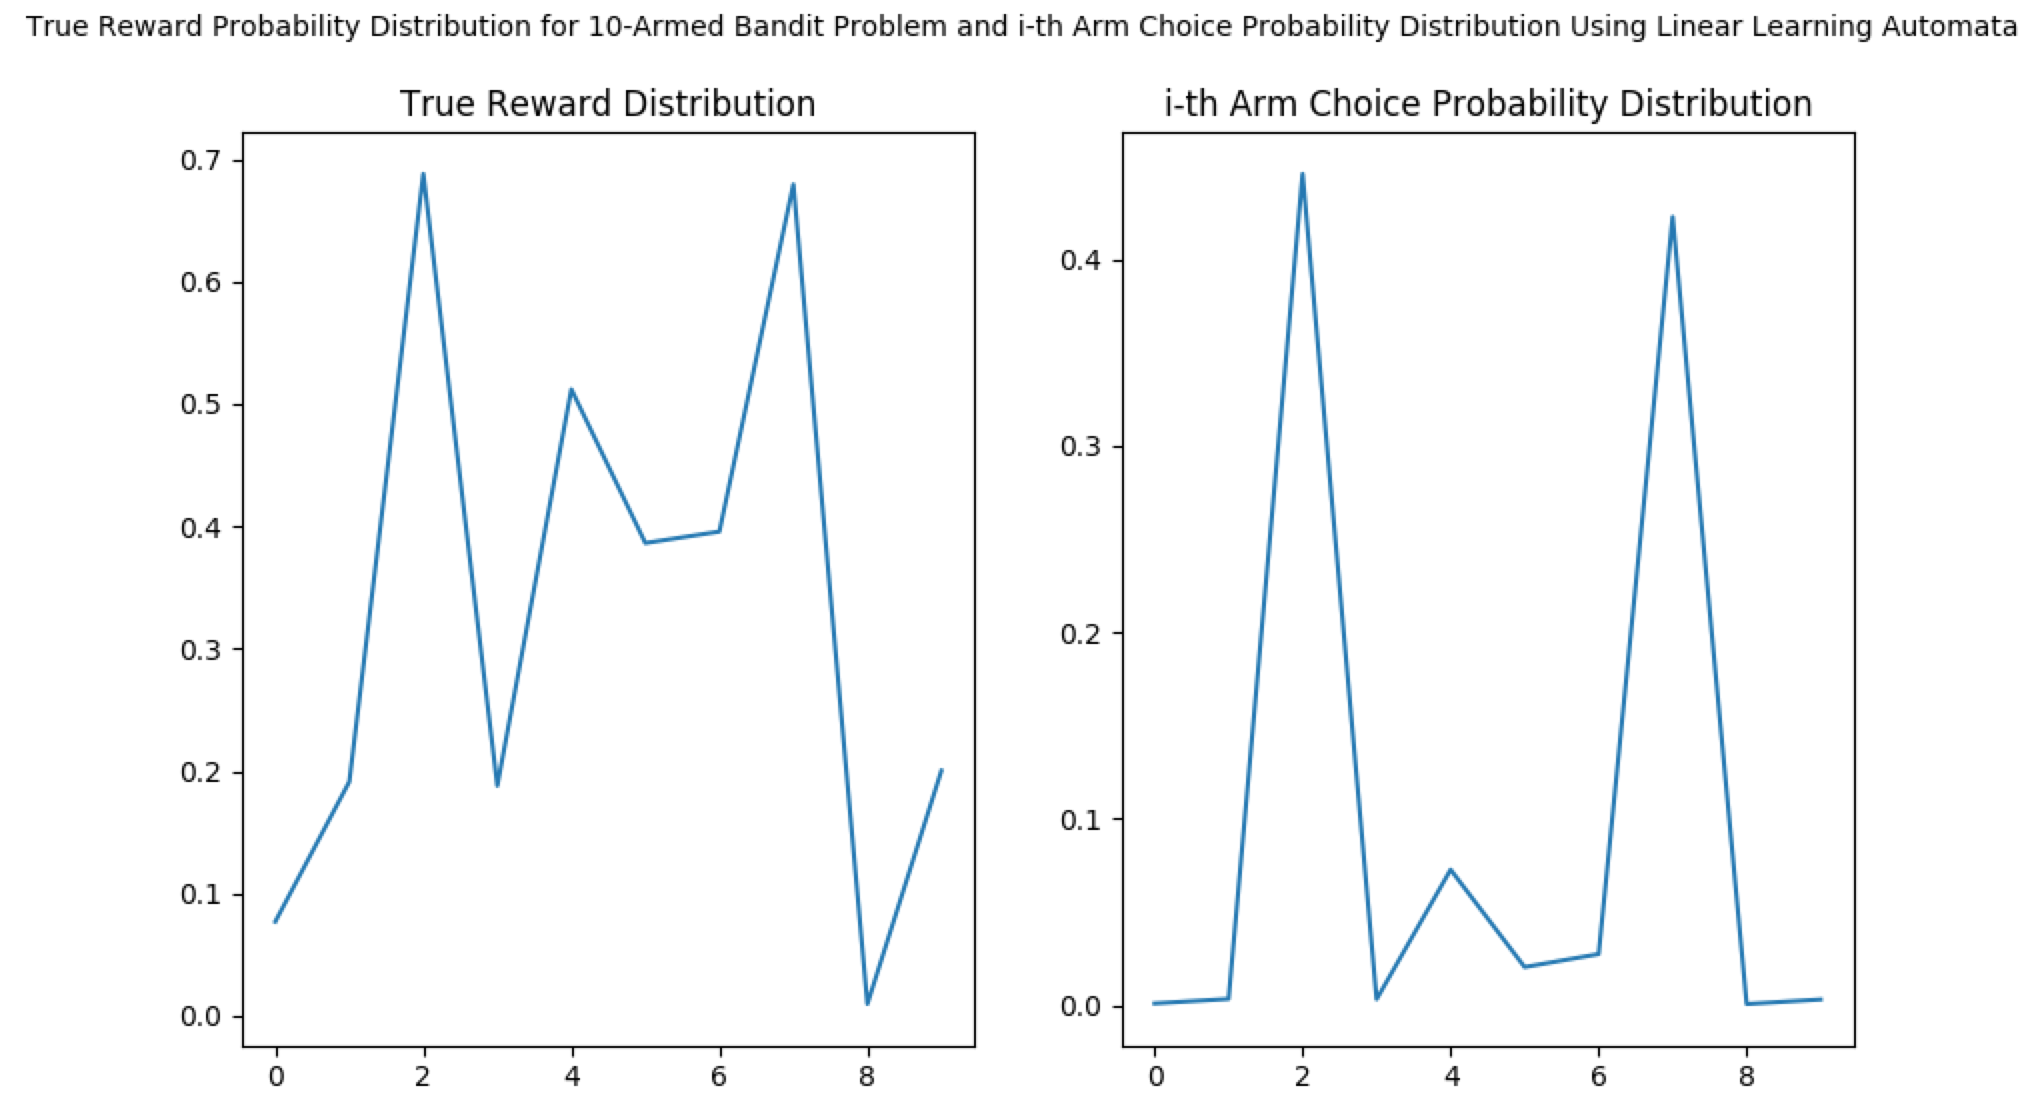
\includegraphics[scale=0.2]{lla_pred_llr}
	\caption{The probability distribution of actions taken by Linear Learning Automata with a high learning rate ($\alpha=1$, top) and that of actions taken by one with a low learning rate ($\alpha=0.0001$, bottom).}
	\end{figure}
	
	It's evident that with a low enough learning rate convergence is more sure to be optimal though slow, while a high learning can force a non-optimal solution, but convergence occurs very quickly.
	

	\item Non-linear automata were more stochastic in their decision making than linear automata, but both were more stochastic in their decision making than the UCB algorithm. The probability distributions of the arms made it such that action selection varied strongly (depending on learning rate as well). A high learning rate often led to the policy collapsing on to one action, causing the optimal action to never being taken, and averaging a reward value depending on that action. This can be seen in Figure 6 and 7.
	
	\begin{figure}[h]
	\centering
	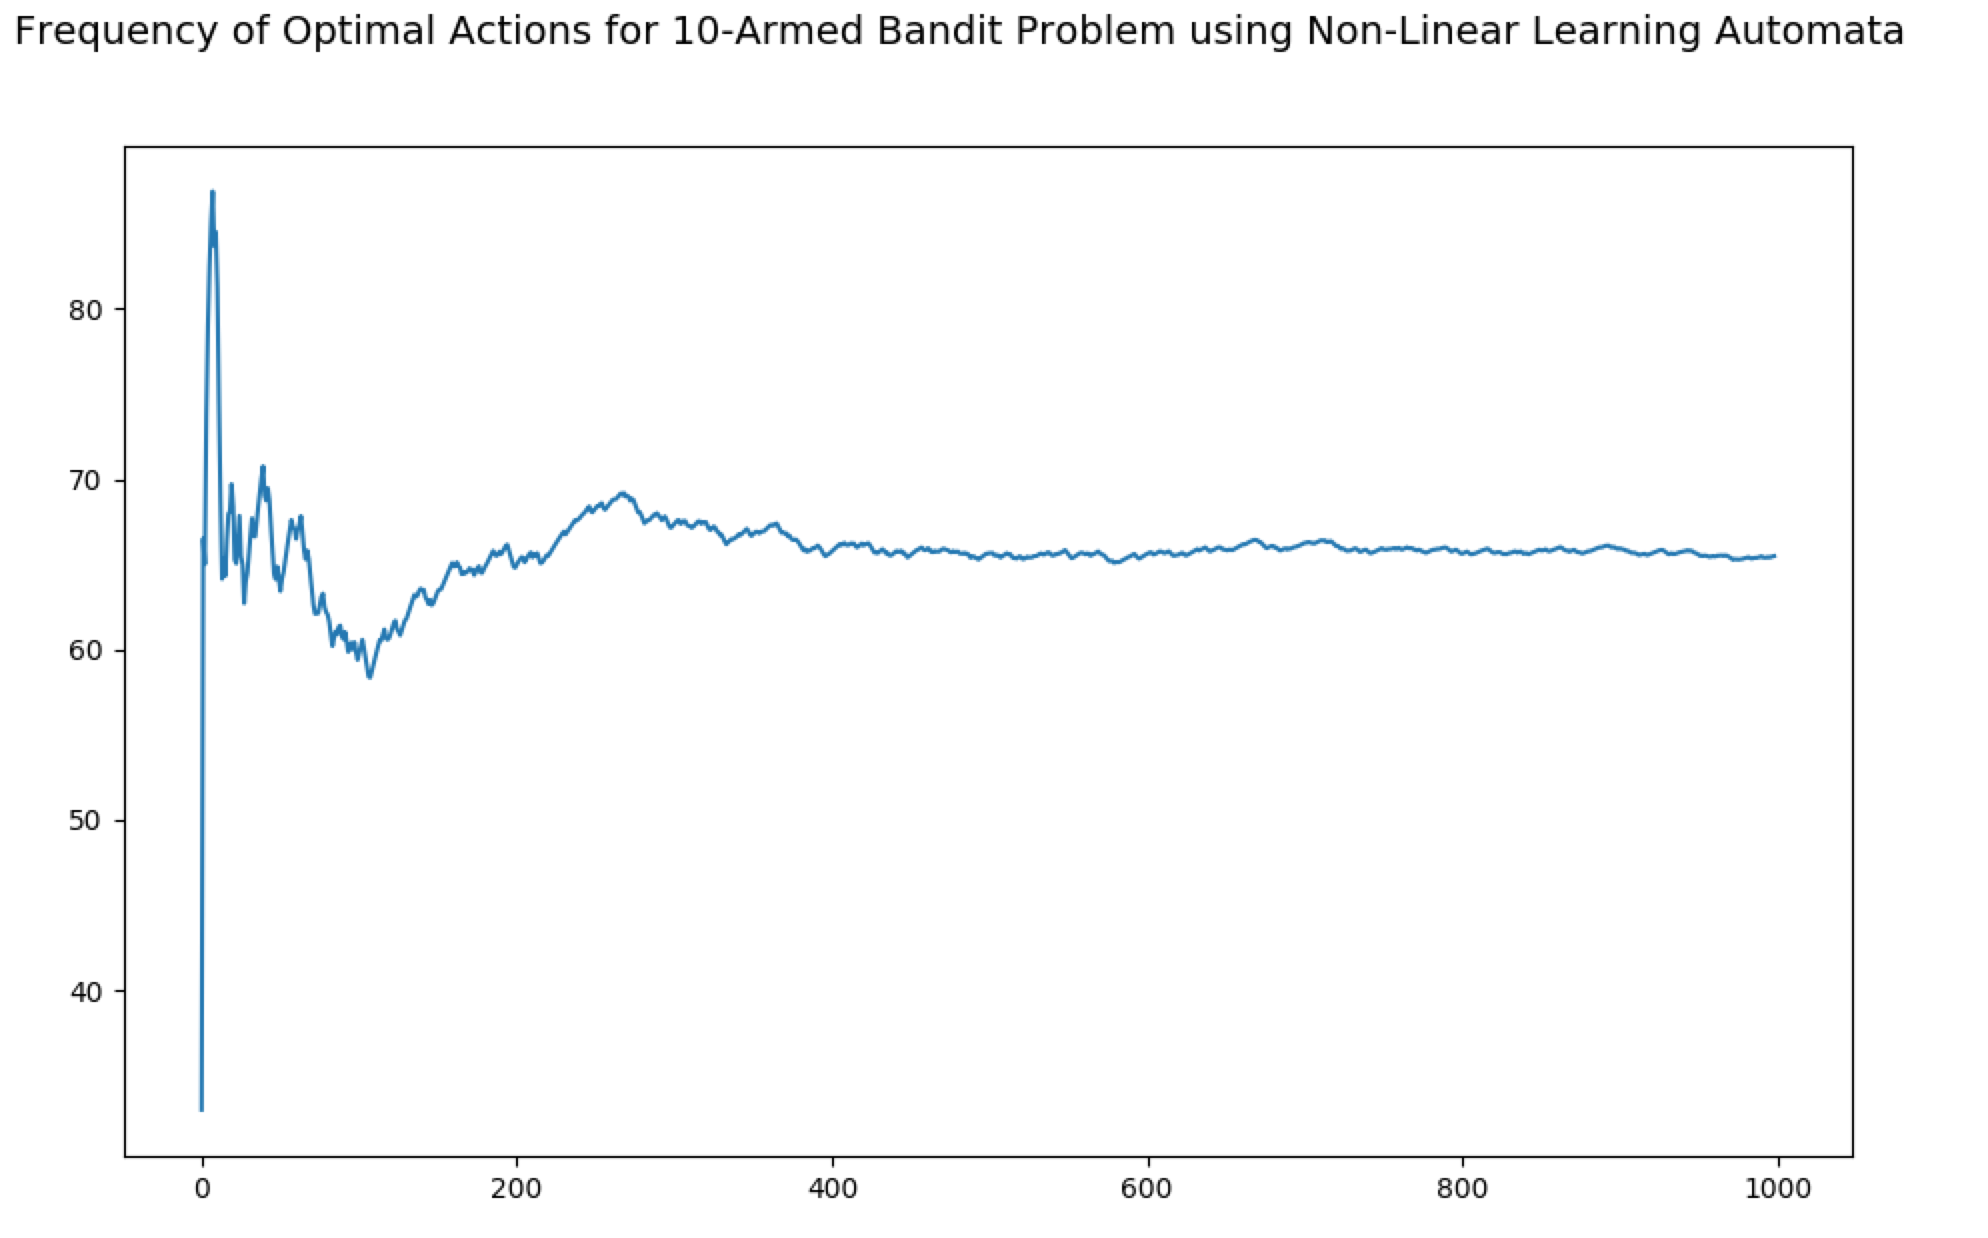
\includegraphics[scale=0.2]{nlla_opt_hlr}
	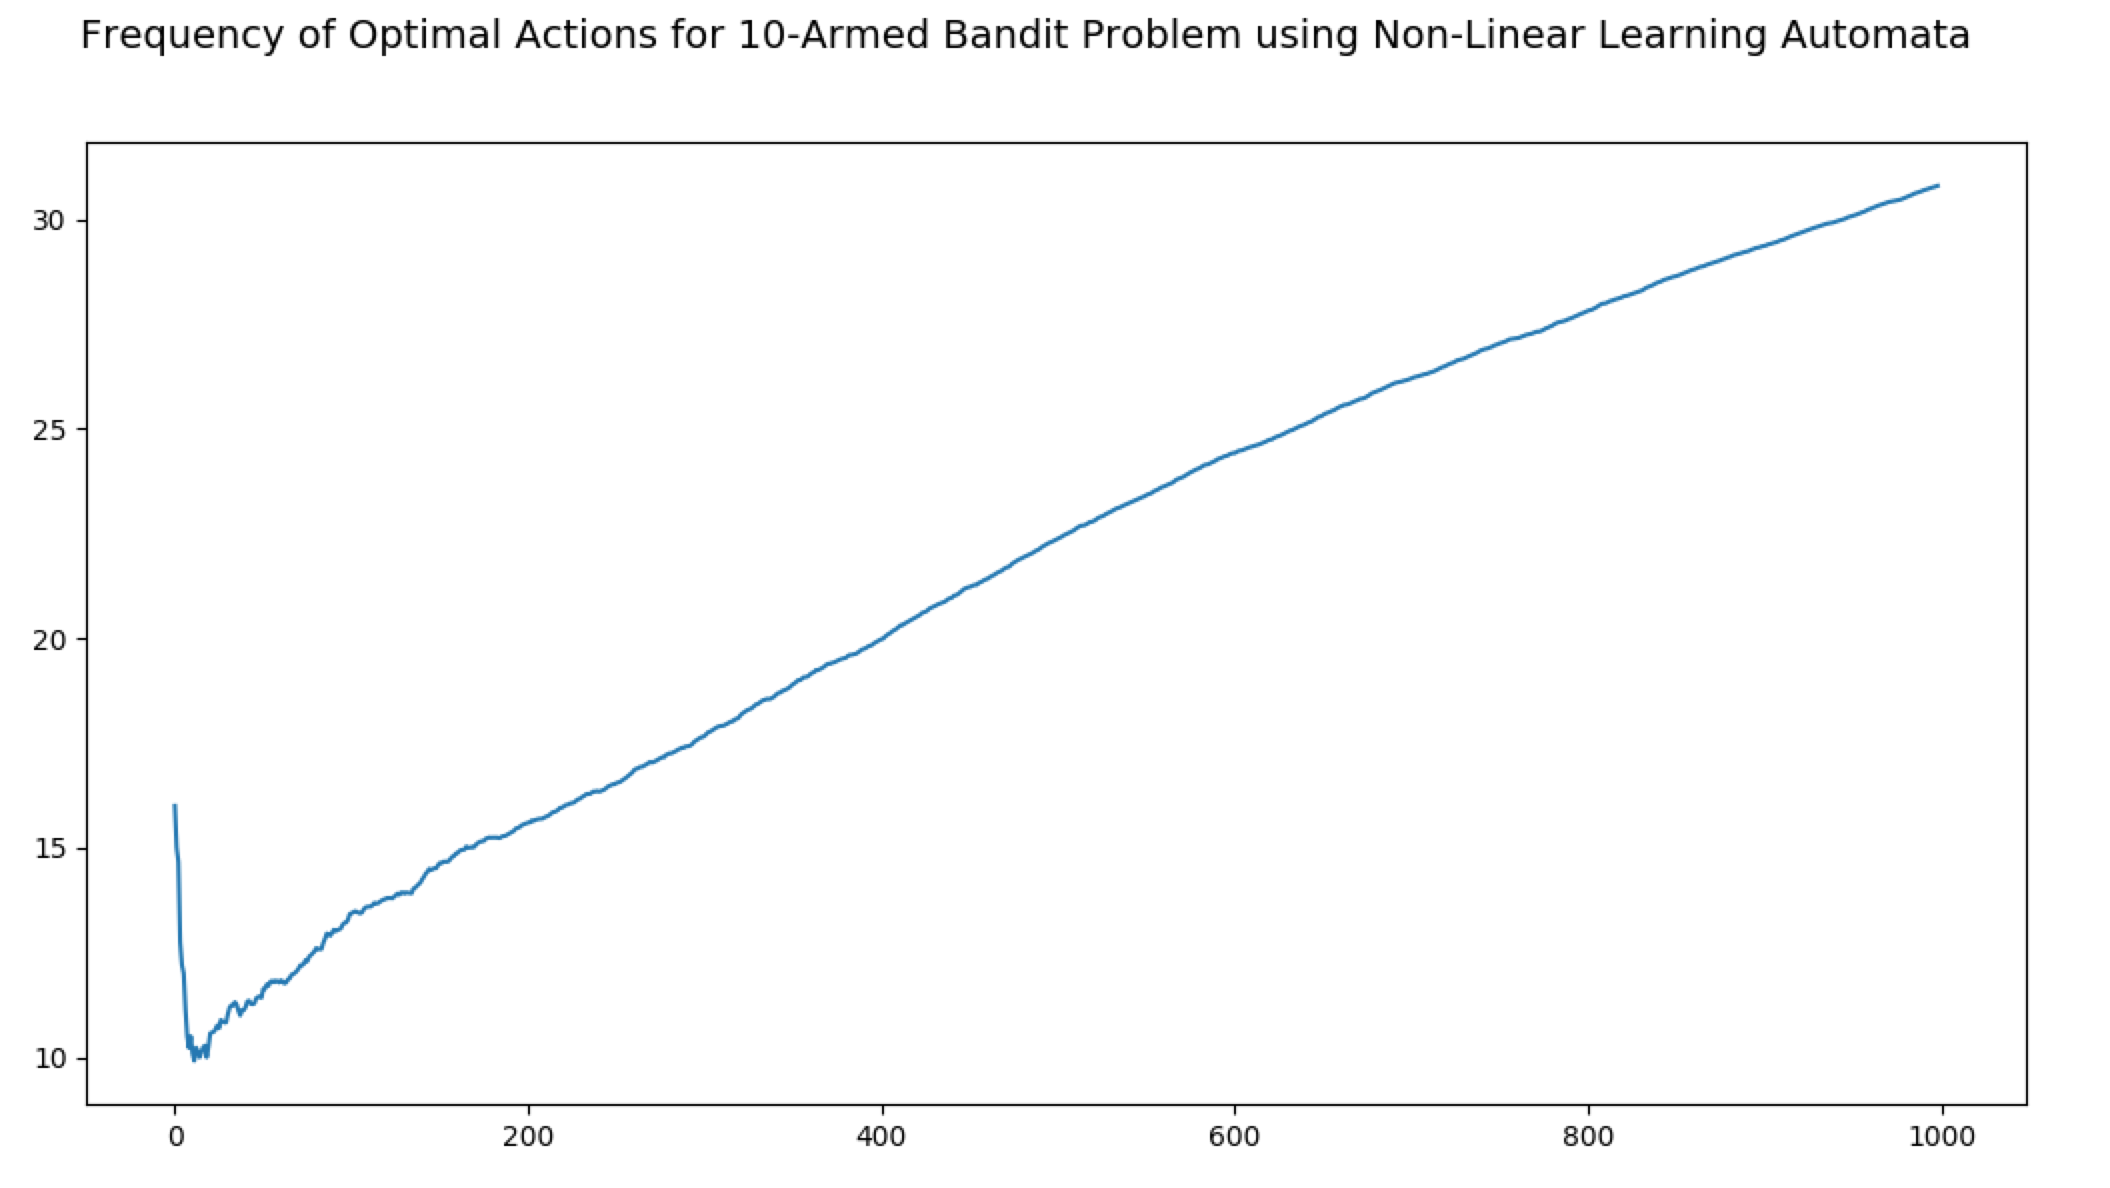
\includegraphics[scale=0.2]{nlla_opt_llr}
	\caption{The optimal moves taken by Non-Linear Learning Automata with a high learning rate ($\alpha=1$, top) and that of actions taken by one with a low learning rate ($\alpha=0.0001$, bottom).}
	\end{figure}
	
	\begin{figure}[h]
	\centering
	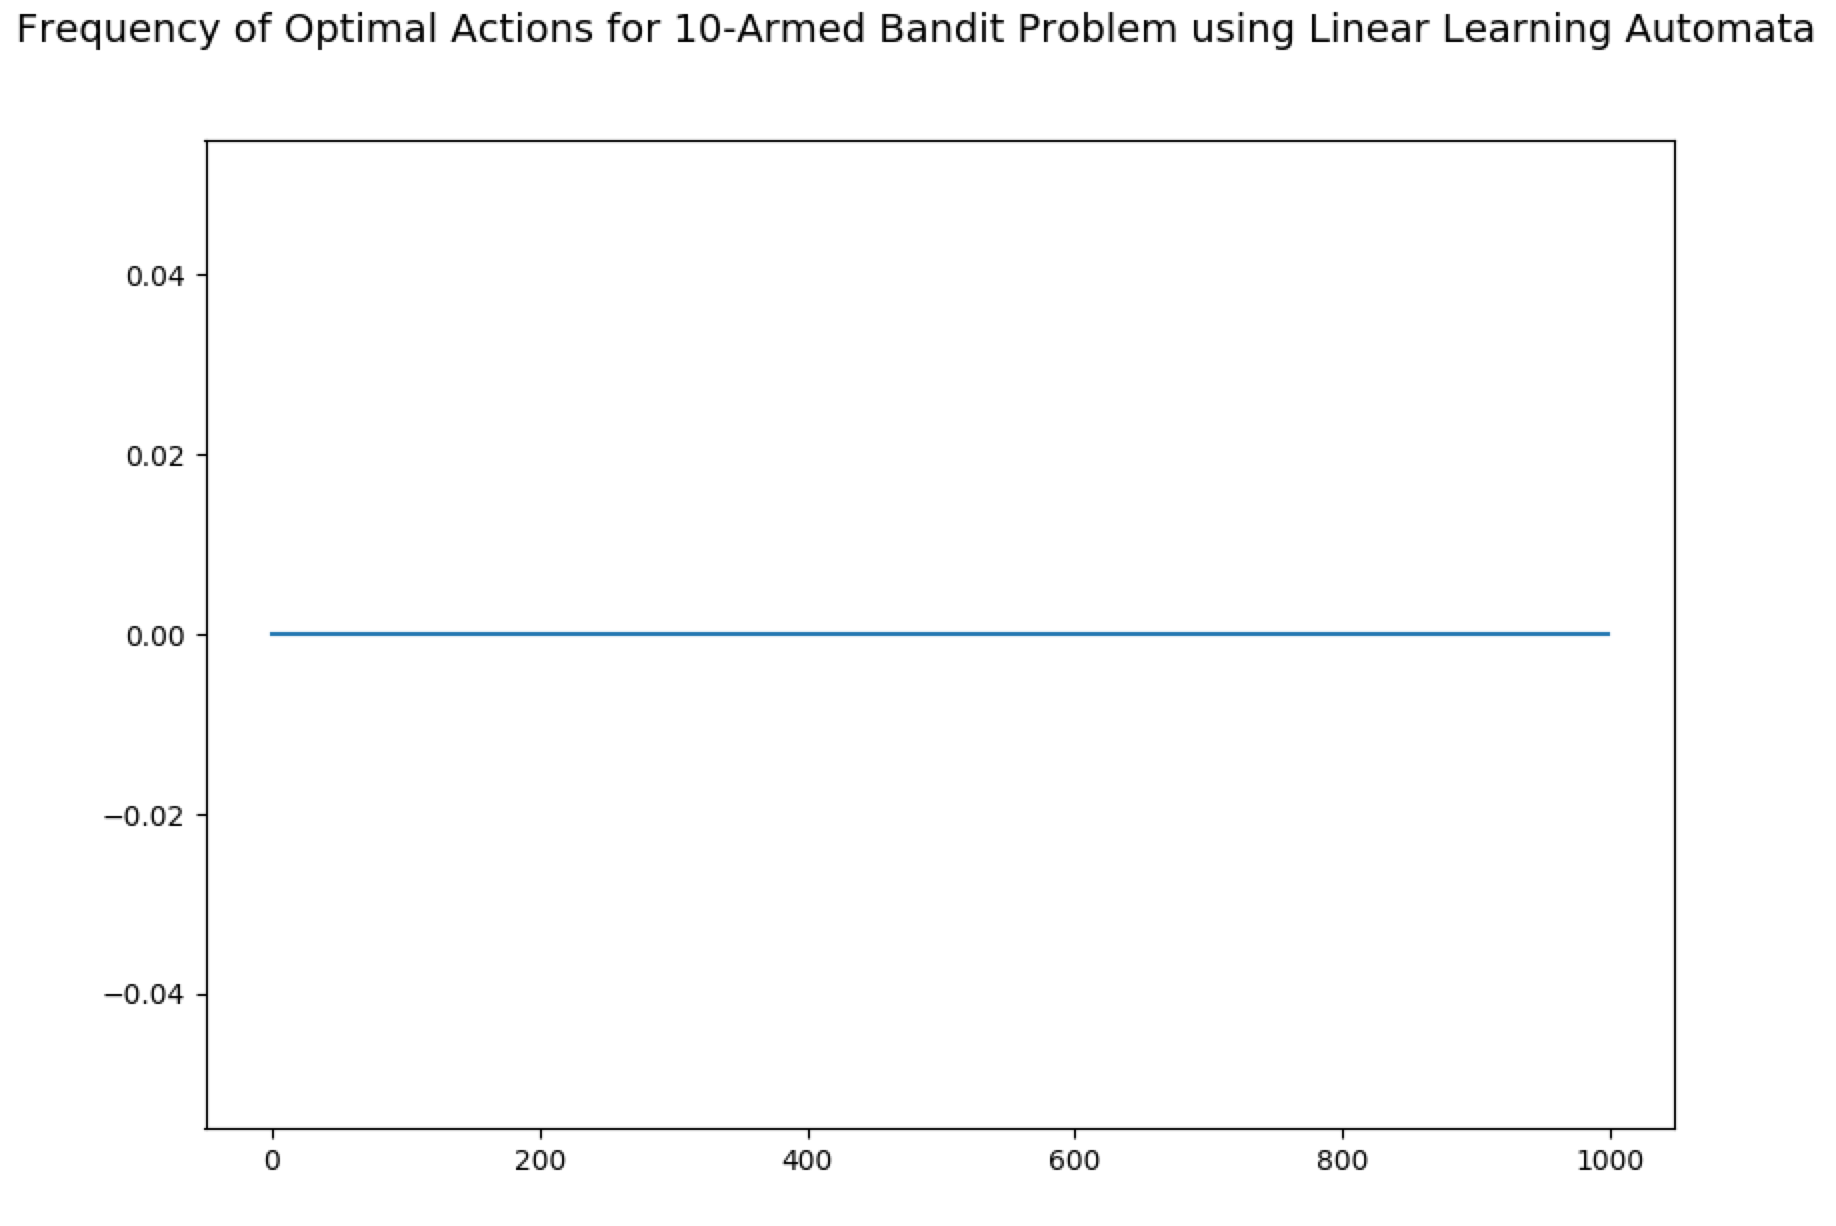
\includegraphics[scale=0.2]{lla_opt_hlr}
	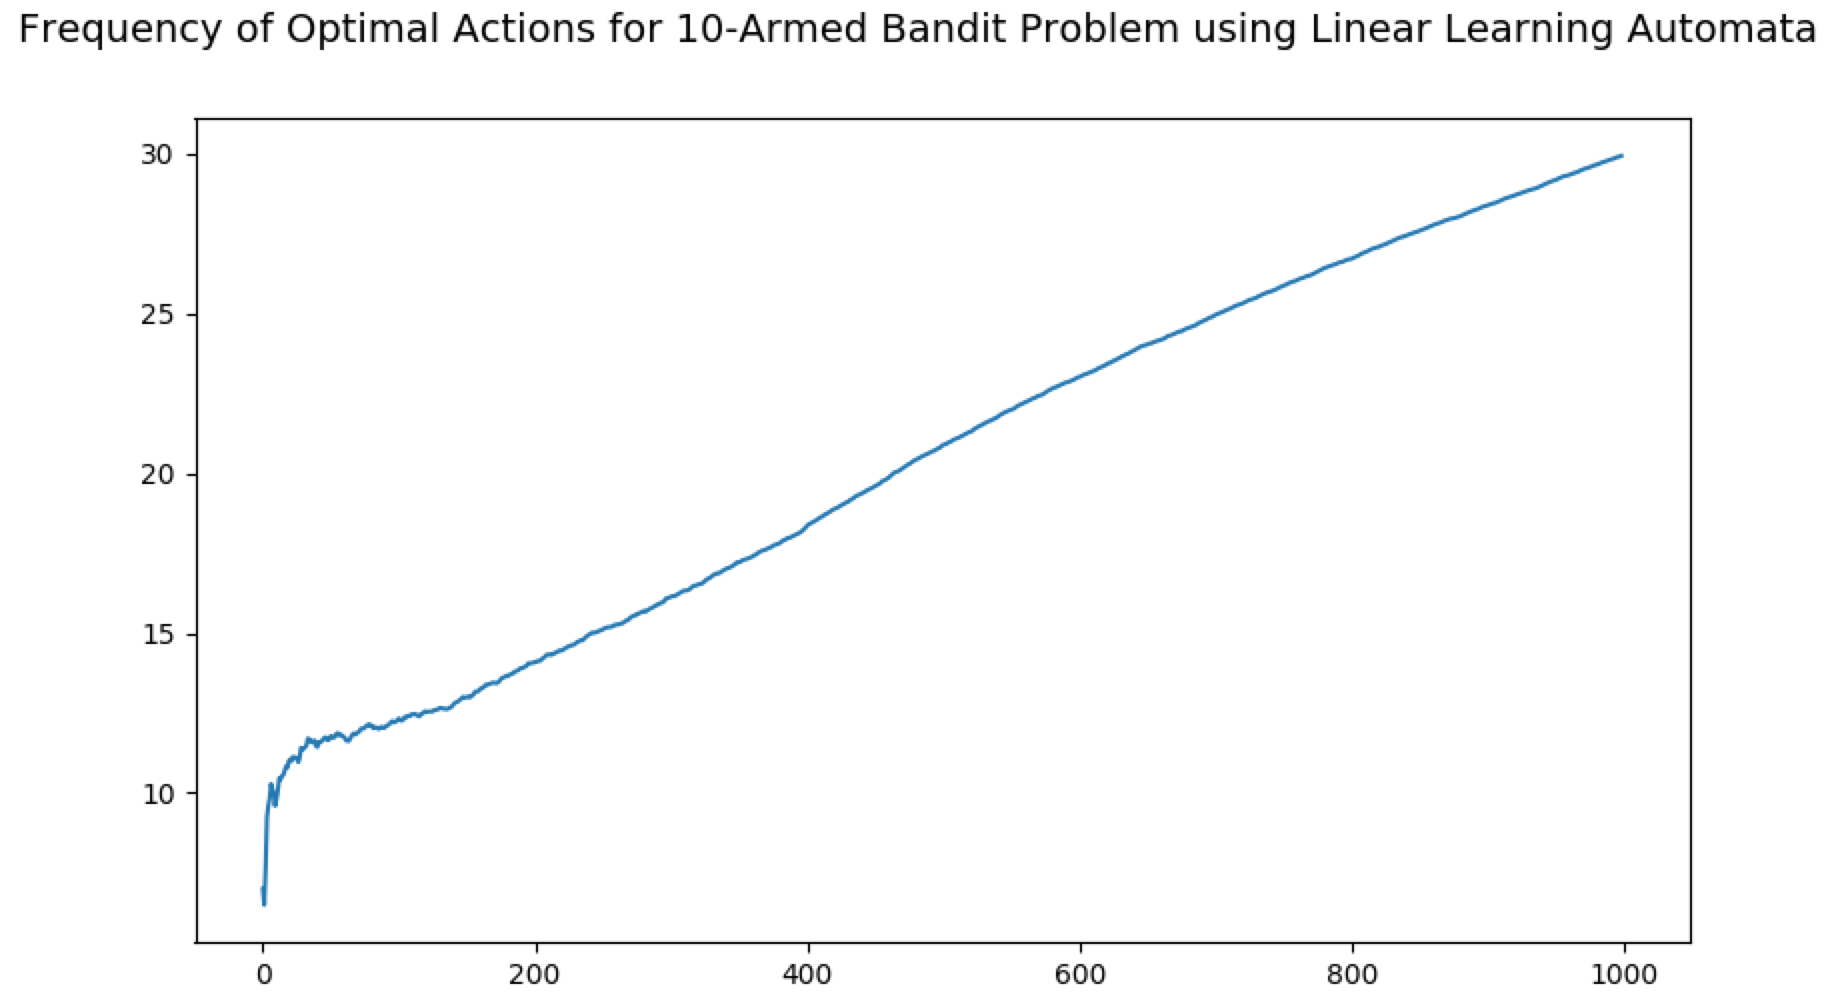
\includegraphics[scale=0.2]{lla_opt_llr}
	\caption{The optimal moves taken by Linear Learning Automata with a high learning rate ($\alpha=1$, top) and that of actions taken by one with a low learning rate ($\alpha=0.0001$, bottom).}
	\end{figure}
	
	\end{enumerate}
	Conclusion: The UCB and Learning Automata can both model simple reinforcement learning tasks. While Learning Automata provide the ability for a stochastic method of action selection with the learning rate $\alpha$ parameter, a similar parameter can be modeled with the UCB algorithm using the $c$ in $A_t = \argmax_x [Q_t(a) + c\sqrt{\frac{lnt}{N_t(a)}}]$. While using Learning Automata could provide an action selection distribution that correlates more strongly with the probability distribution of rewards, it seems pointless to focus on accurately modeling the non-optimal moves in the 10-arm bandit problem. That is, if the optimal move is known, the sub-optimal moves should not be made. The UCB algorithm provides this by allowing for a measure of degree of uncertainty that decreases over time. It also generally converges to a value quicker than either the linear or non-linear learning automata.
	
	
	
	
\end{document}